\subsection{Application Design}

The tool we implemented is designed as pipeline that takes an arbitrary database as input and outputs a set of SQL scripts, which can be run to create a new database having a dimensional scheme.
The user is guided throughout the whole process via a command line interface, which enforces him to do the steps in the right order.
As a special feature we implemented a mechanism to save the current working state in order to continue the work at a later point in time.
As soon as all the specifications about the resulting scheme are made, the program will output and run the resulting SQL scripts in a way that the new database is created and the original data is populated.

\paragraph{Making suggestions}

The program tries to support the user in a helpful way.
After the input database scheme is read, the system will come up with some suggestions for the categorization of tables (according to \ref{par:classifyEntities}).

Since it is a hard job to find transaction candidates without knowing about the business from only the database schema, we decided to use a different approach.
It is likely that the user will choose a minimal entity as transaction because it is one of the roots of the database and therefore a very important table for the business.
In order to obtain every minimal entity we find every table that is not referenced by any foreign key.


\paragraph{User interaction}

- generation can not be done completely automatically
- users needs and desires are unpredictable and the according structure of dimensional as well
- therefore we need user interaction and the supervision and confirmation of the user
- every time a suggestion is made by the program, it will be presented to the user, letting him modify this shit and confirm when he thinks the right design is chosen.

SaveAndLoad

\paragraph{Generating SQL}
TODO Dusan %TODO

\subsection{Implementation Details}

\begin{figure}
  \centering
  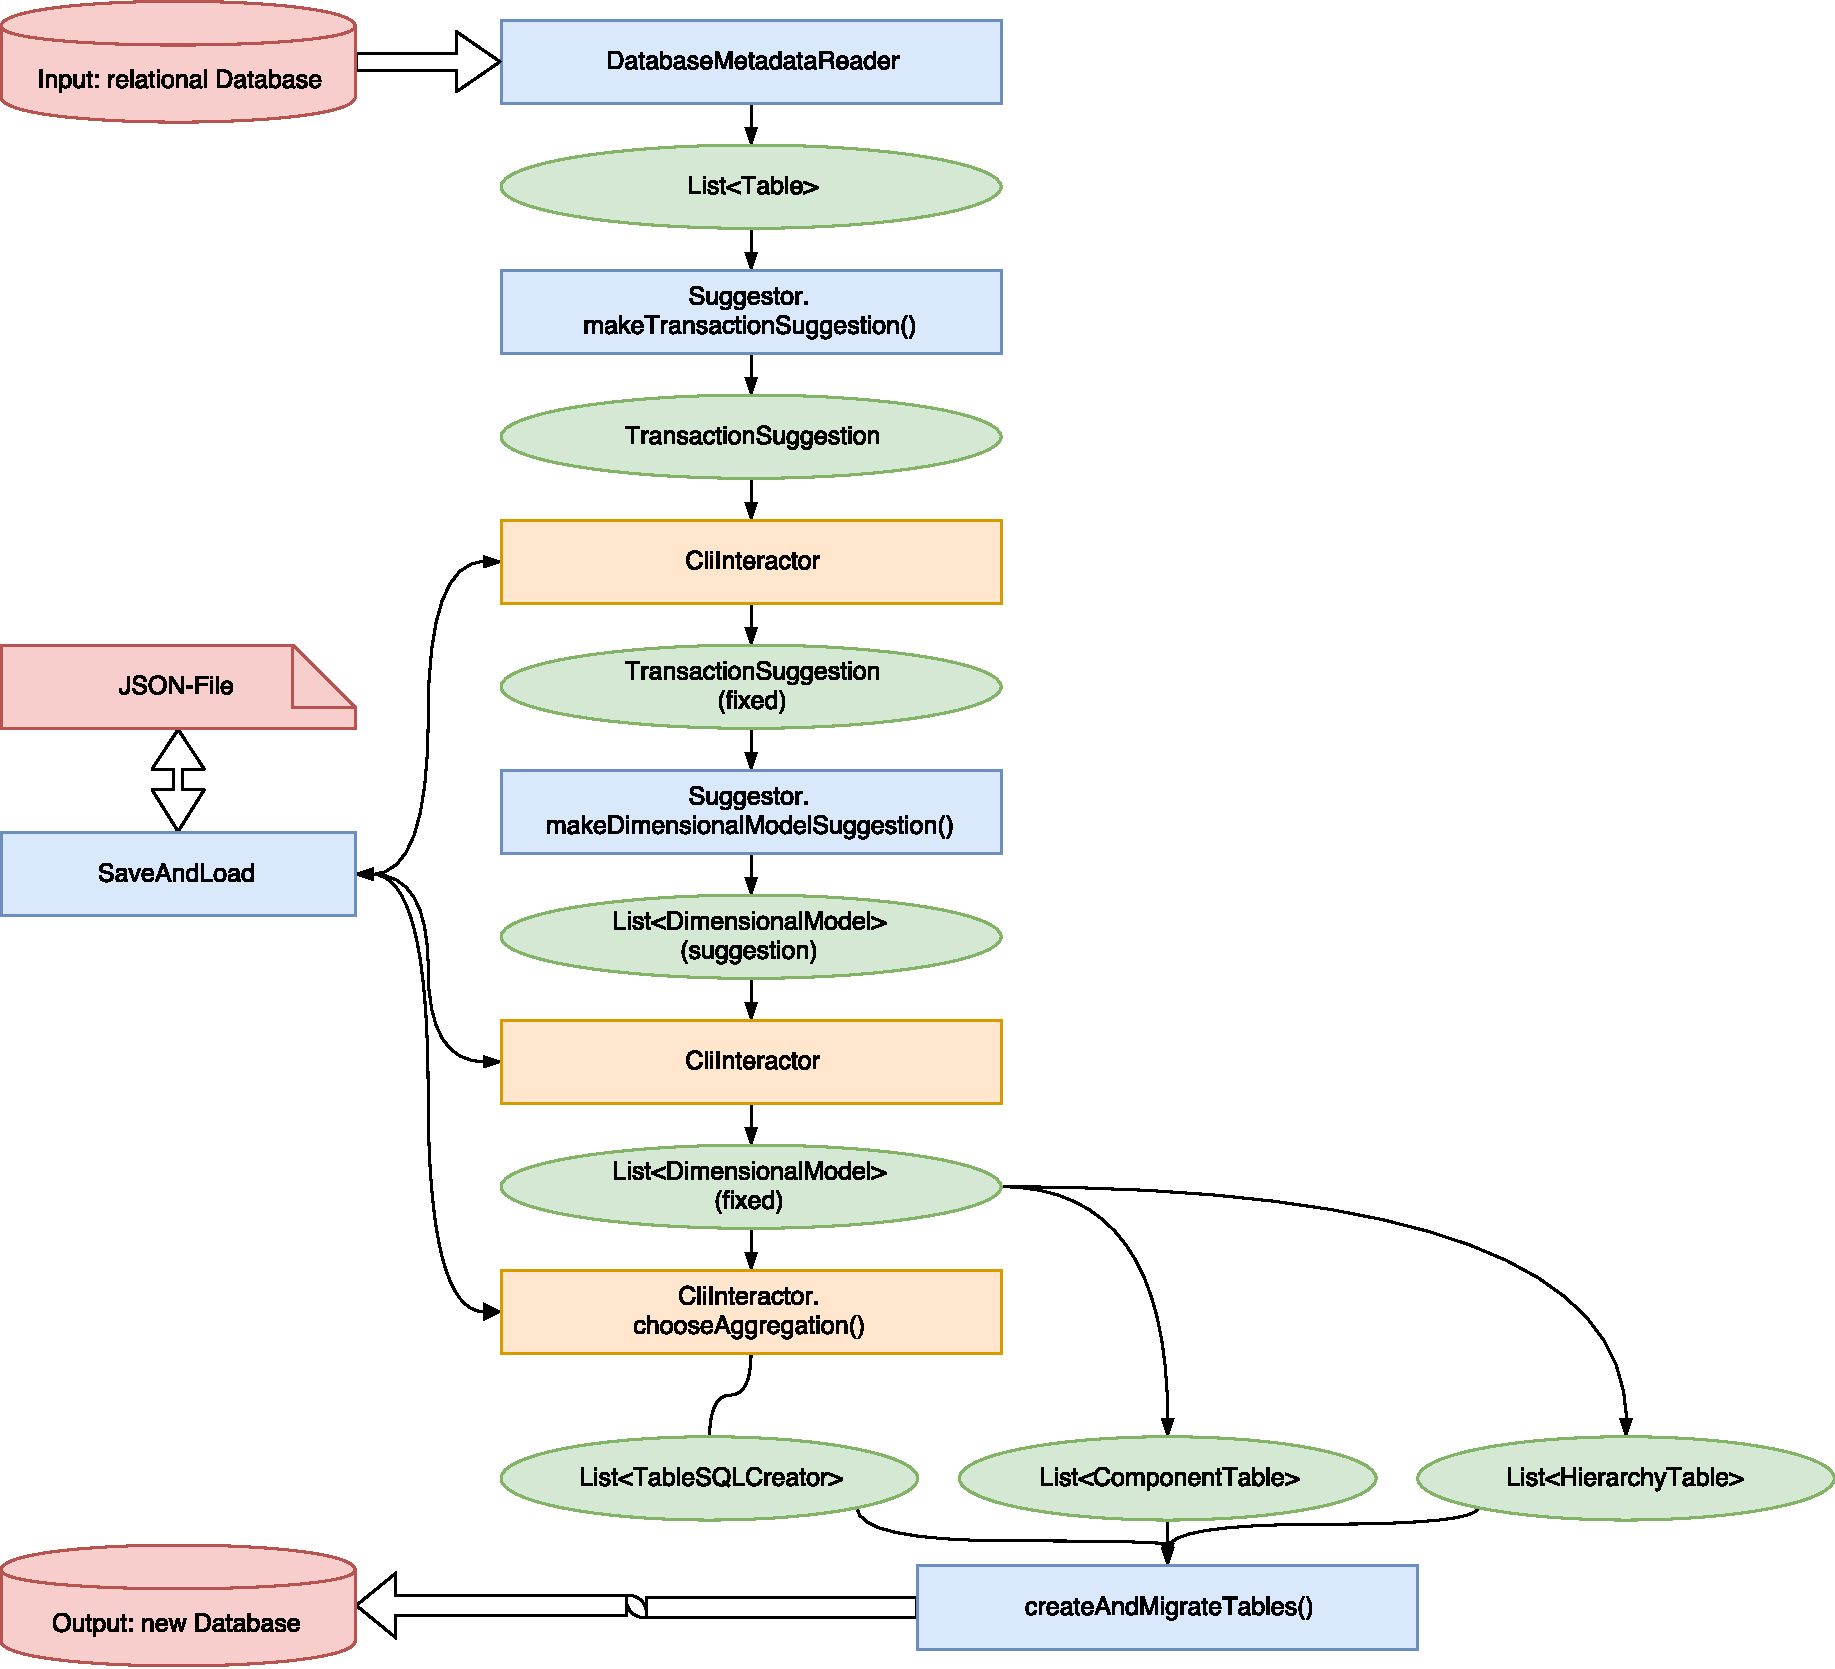
\includegraphics[width=\linewidth]{images/dataFlowDiagram}
  \caption{Dataflow Diagram of the Pipeline.}
  \label{fig:dataflowDiagram}
\end{figure}

As a first step the input database is parsed using the JDBC library\footnote{\url{http://www.oracle.com/technetwork/java/javase/jdbc/index.html}}.

\begin{figure}[p]
  \lstinputlisting[breaklines]{images/metadataOutput.txt}
  \caption{Output of parsed metadata}
  \label{fig:metadataOutput}
\end{figure}

\subsection{Usage of the Tool}

\begin{figure}[p]
  \lstinputlisting[breaklines]{images/transactionSuggestion.txt}
  \caption{Commandline interface: Suggestion and Selection of \emph{Transaction entities}}
  \label{fig:transactoinSuggestion}
\end{figure}

\begin{figure}[p]
  \lstinputlisting[breaklines]{images/dimensionalModelSuggestion.txt}
  \caption{Commandline interface: Suggestion and Selection of \emph{Component and Classification entities}}
  \label{fig:dimensionalModelSuggestion}
\end{figure}

\begin{figure}[p]
  \lstinputlisting[breaklines]{images/aggregationSelection.txt}
  \caption{Commandline interface: Selection of \emph{Aggregation functions}}
  \label{fig:aggregationSelection}
\end{figure}

